Triangles are the fundamental shapes that make up (literally) much of geometry. The purpose of this lecture is not to provide a rigorous, in-depth treatment of geometry, but rather give formulas and definitions that will aid a student in solving competition math problems. Keep in mind that the material in this lecture ranges from introductory to intermediate, so it covers a wide range of difficulties. This lecture is partly adpated from Jennifer Yin's ``Triangles!'' lecture from TJ VMT ARML practice on March 7, 2013.
\subsection{Special Properties of Triangles}
There are lines and points on triangles that have special properties:
\begin{enumerate}
    \item \textbf{Medians:} These intersect the sides of a triangle at their midpoints; their common point of intersection is called the \textbf{centroid}. An important property of medians is that the length of a centroid to a vertex is always twice that of its distance to the opposite side.
    \item \textbf{Angle Bisectors:} These are the lines of a triangle that bisect the angles of a triangle. The angle bisectors of a triangle intersect at a common point called the triangle's \textbf{incenter}, which is the center of the triangle's \textbf{incircle} (a circle that can be inscribed inside the triangle that is tangent to all three sides).
    \item \textbf{Perpendicular Bisectors:} These lines perpendicularly bisect the sides of the triangle. Their common point of intersection is called the \textbf{circumcenter}, which is the center of the triangle's \textbf{circumcircle}.
    \item \textbf{Altitudes:} These intersect at a common point called the triangle's \textbf{orthocenter}. Problems that involve altitudes typically use the Pythagorean theorem.
\end{enumerate}

\clearpage
\subsection{Formulas for the Triangle}
All of these theorems have proofs that you can look up. Some are easy to prove, but others can be very difficult. Although it's important to understand how some of them are derived, it is not necessary to know them in order to solve problems.
\subsubsection{Side Lengths}
\begin{itemize}
    \item \textbf{Pythagorean Theorem:} $\displaystyle a^2+b^2=c^2$, where $c$ is the hypotenuse and $a, b$ are the two legs of a \textit{right triangle}. Arguably one of the most basic and important equations you'll need to know.
    \item \textbf{Angle Bisector Theorem:} If $\bigtriangleup ABC$ has an angle bisector from $A$ that intersects $BC$ at  $D$, then $\displaystyle \frac{AB}{BC} = \frac{AC}{CD}$ 
    \item \textbf{Law of Cosines: } $\displaystyle c^2 = a^2+b^2-2ab\cos\theta$, where $\theta=\angle ACB$ (the angle at $C$).
    \item \textbf{The Law of Sines: } $\displaystyle \frac{a}{\sin A} = \frac{b}{\sin B} = \frac{c}{\sin C} = 2R$, where $a$ denotes side $BC$ and $A$ denotes the angle at $A$.
    \item \textbf{Stewart's Theorem:} $b^2m + c^2n = a(d^2 + mn)$ This theorem works for any cevian $AD$ of $\bigtriangleup ABC$. This theorem is better remembered as $dad+man=bmb+cnc$, which (if you use your imagination), can be read as ``Dad and man put a bomb in the sink.''
    \begin{center}
    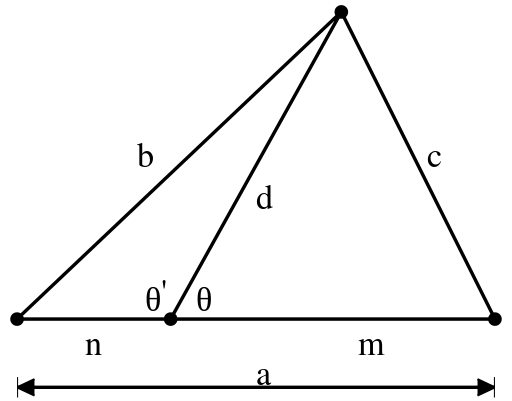
\includegraphics[width = 2in]{stewarts}
    \end{center}
    \item \textbf{Ceva's Theorem:} $\frac{AF}{AE} = \frac{BD}{BF} = \frac{CE}{CD} = 1$, where $\bigtriangleup ABC$ has points $D, E, F$ on sides $BC, AC, AB$ respectively, and cevians $AD, BE, CF$ are concurrent at a single point.
\end{itemize}
\subsubsection{Area}
Let $K$ be the area of $\bigtriangleup ABC$, then:
\begin{itemize}
    \item $\displaystyle K = \frac{1}{2}bh$, where $b$ is the base and $h$ is the height
    \item $\displaystyle K = \sqrt{s(s-a)(s-b)(s-c)}$, where $s$ is the semiperimeter of $\bigtriangleup ABC$, which is $\frac{a+b+c}{2}$. This is called \textit{Heron's Formula}.
    \item $\displaystyle K = \frac{abc}{4R}$, where $R$ is the radius of the circumcircle
    \item $\displaystyle K = rs$, where $r$ is the radius of the incircle and $s$ is the semiperimeter
    \item $\displaystyle K = \frac{1}{2}ab\sin C$
\end{itemize}

\subsubsection{Remarks}
Keep in mind that although these formulas and theorems work, they don't solve problems directly for you (except in introductory problems). You still have to use your brain, and try to find ways to apply them \textit{only when they are relevant}. Also, this list is obviously not complete (there are hundreds of theorems out there), but hopefully this gives you a stepping stone into geometry for the AMCs and other competition math.

\subsection{Problems}
\begin{problem}
An equilateral triangle and a regular hexagon have equal perimeters. If the area of the triangle is 4, what is the area of the hexagon? \vspace{0.2in}

$\textbf{(A)}\hspace{.05in}4\qquad\textbf{(B)}\hspace{.05in}5\qquad\textbf{(C)}\hspace{.05in}6\qquad\textbf{(D)}\hspace{.05in}4\sqrt3\qquad\textbf{(E)}\hspace{.05in}6\sqrt3$
\end{problem} 

\begin{problem}
The base of an isosceles triangle is $6$ inches and one of the equal sides is $12$ inches. What is the radius of the circle through the vertices of the triangle? \vspace{0.2in}

$\textrm{(A) } 2 \qquad \textrm{(B) } \frac{4 \sqrt {3}}{3} \qquad \textrm{(C) } \frac{5\sqrt{3}}{3} \qquad \textrm{(D) } \frac{8\sqrt{15}}{5} \qquad \textrm{(E) } 6 \sqrt {3}$
\end{problem}

\begin{problem}
Equilateral $\triangle ABC$ has side length $1$, and squares $ABDE$, $BCHI$, $CAFG$ lie outside the triangle. What is the area of hexagon $DEFGHI$?
\begin{center}
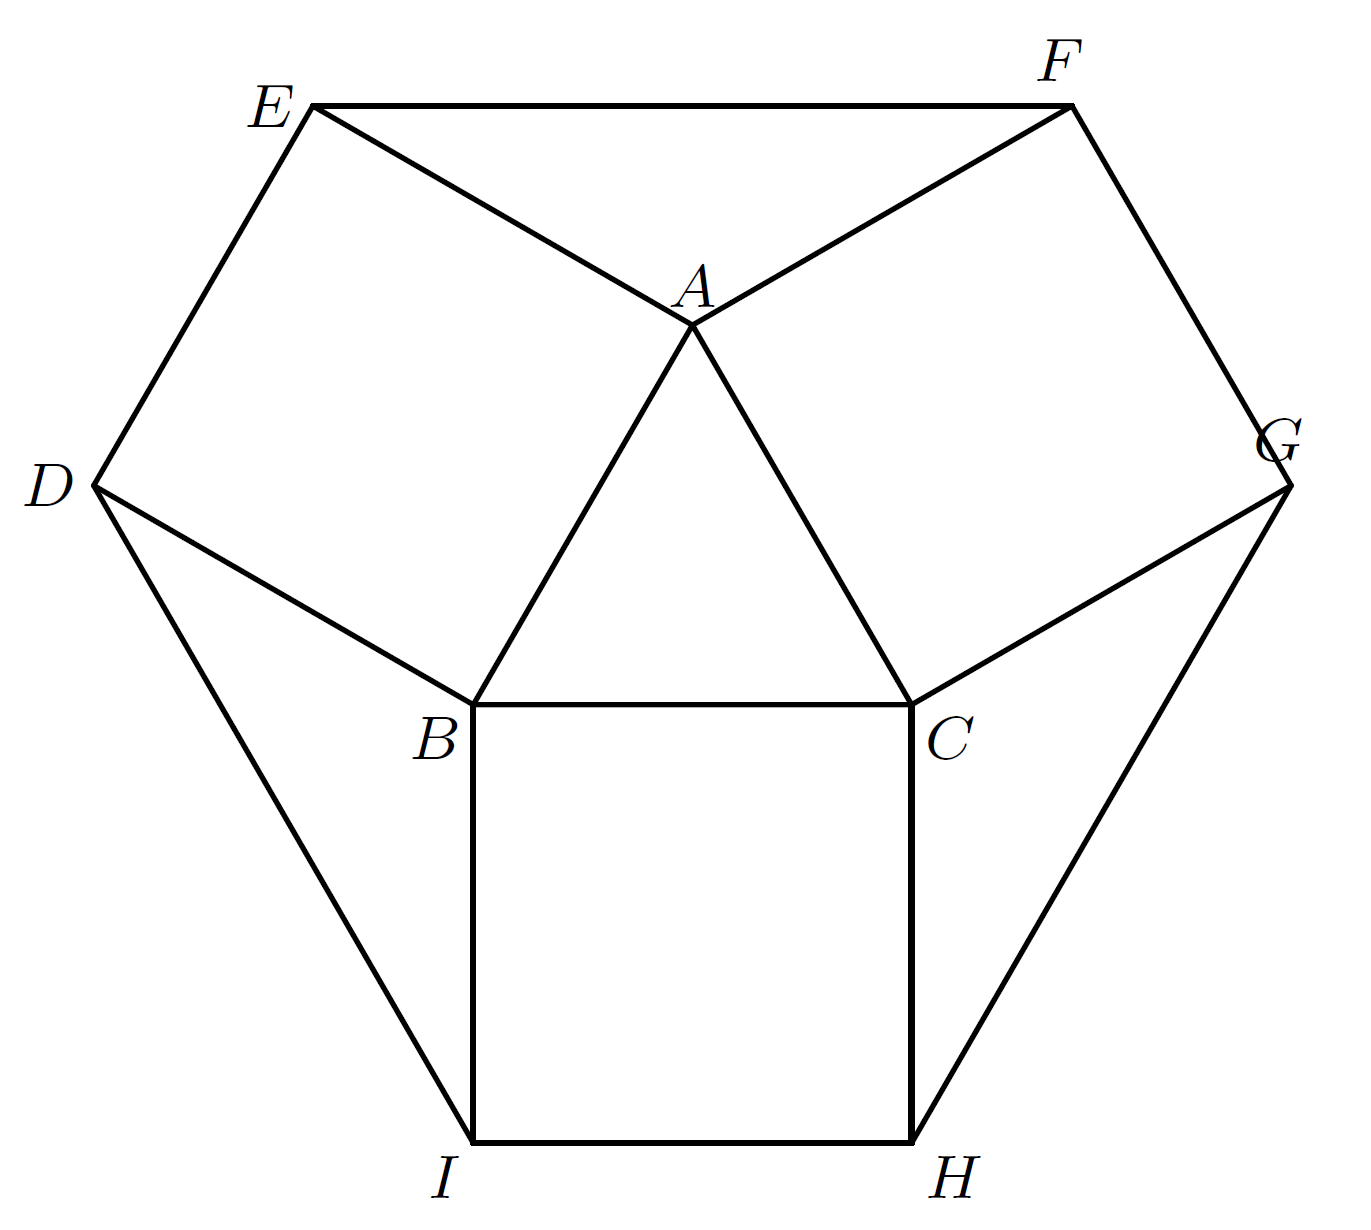
\includegraphics[height=2in]{hex}
\end{center}
$\textbf{(A)}\ \dfrac{12+3\sqrt3}4\qquad\textbf{(B)}\ \dfrac92\qquad\textbf{(C)}\ 3+\sqrt3\qquad\textbf{(D)}\ \dfrac{6+3\sqrt3}2\qquad\textbf{(E)}\ 6$
\end{problem}

\begin{problem}
Rhombus $ABCD$ is similar to rhombus $BFDE$. The area of rhombus $ABCD$ is 24, and $\angle BAD = 60^\circ$. What is the area of rhombus $BFDE$?
 \begin{center}
    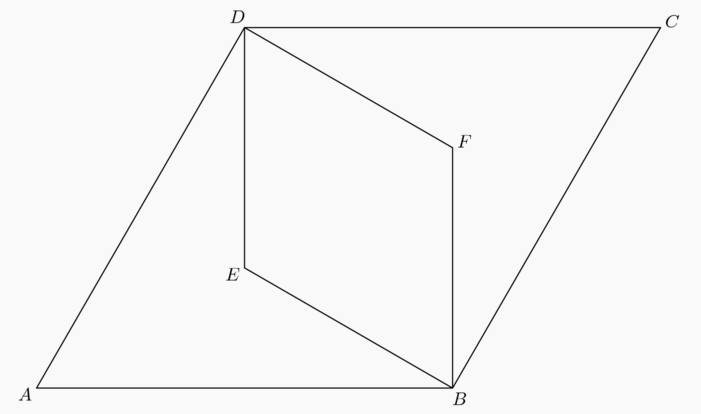
\includegraphics[width = 3in]{rhombus}
    \end{center}
$\textrm{(A) } 6 \qquad \textrm{(B) } 4\sqrt {3} \qquad \textrm{(C) } 8 \qquad \textrm{(D) } 9 \qquad \textrm{(E) } 6\sqrt {3}$
\end{problem}

\begin{problem}
Three congruent isosceles triangles are constructed with their bases on the sides of an equilateral triangle of side length $1$. The sum of the areas of the three isosceles triangles is the same as the area of the equilateral triangle. What is the length of one of the two congruent sides of one of the isosceles triangles? \vspace{0.2in}

$\textbf{(A) }\dfrac{\sqrt3}4\qquad \textbf{(B) }\dfrac{\sqrt3}3\qquad \textbf{(C) }\dfrac23\qquad \textbf{(D) }\dfrac{\sqrt2}2\qquad \textbf{(E) }\dfrac{\sqrt3}2$
\end{problem}

\begin{problem}
In triangle $ABC$, $AB = 13$, $BC = 14$, $AC = 15$. Let $D$ denote the midpoint of $\overline{BC}$ and let $E$ denote the intersection of $\overline{BC}$ with the bisector of angle $BAC$. Which of the following is closest to the area of the triangle $ADE$? \vspace{0.2in}

$\text {(A)}\ 2 \qquad \text {(B)}\ 2.5 \qquad \text {(C)}\ 3 \qquad \text {(D)}\ 3.5 \qquad \text {(E)}\ 4$
\end{problem}

\begin{problem}
A right triangle has perimeter $32$ and area $20$. What is the length of its hypotenuse? \vspace{0.2in}

$\mathrm{(A)}\ \frac{57}{4}\qquad\mathrm{(B)}\ \frac{59}{4}\qquad\mathrm{(C)}\ \frac{61}{4}\qquad\mathrm{(D)}\ \frac{63}{4}\qquad\mathrm{(E)}\ \frac{65}{4}$
\end{problem}

\begin{problem}
A circle centered at $O$ has radius $1$ and contains the point $A$. The segment $AB$ is tangent to the circle at $A$ and $\angle AOB = \theta$. If point $C$ lies on $\overline{OA}$ and $\overline{BC}$ bisects $\angle ABO$, then $OC =$
\begin{center}
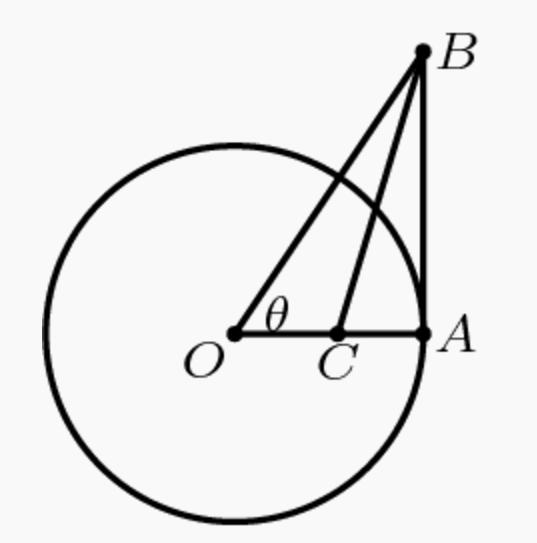
\includegraphics[width=2in]{circle}
\end{center}
$\text {(A)}\ \sec^2 \theta - \tan \theta \qquad \text {(B)}\ \frac 12 \qquad \text {(C)}\ \frac{\cos^2 \theta}{1 + \sin \theta}\qquad \text {(D)}\ \frac{1}{1+\sin\theta} \qquad \text {(E)}\ \frac{\sin \theta}{\cos^2 \theta}$
\end{problem}